%(BEGIN_QUESTION)
% Copyright 2010, Tony R. Kuphaldt, released under the Creative Commons Attribution License (v 1.0)
% This means you may do almost anything with this work of mine, so long as you give me proper credit

Examine this ladder diagram for a solenoid valve control circuit, where the status of a solenoid valve (either on or off) is controlled by hand switches and a pressure switch.  Then, answer the questions that follow:

$$\includegraphics[width=15.5cm]{i04152x01.eps}$$

\begin{itemize}
\item{} Identify the meaning of the square boxes (each one with a unique number inside)
\vskip 10pt
\item{} Identify the three positions of the {\it Hand/Off/Auto} switch and the meaning of each one
\vskip 10pt
\item{} Explain why diodes are found in parallel with the solenoid and relay coils, but not in parallel with the lamp
\vskip 10pt
\item{} Identify the meaning of the numbers near each side of the relay contacts
\vskip 10pt
\item{} Identify whether the pressure switch enables the solenoid to energize if the sensed pressure {\it exceeds} the trip point or {\it falls below} the trip point
\vskip 10pt
\item{} Identify the meaning of the red indicator light
\end{itemize}

\vskip 20pt \vbox{\hrule \hbox{\strut \vrule{} {\bf Suggestions for Socratic discussion} \vrule} \hrule}

\begin{itemize}
\item{} Explain what would happen if either of the two diodes in this circuit were reversed.
\item{} What would happen if the reset switch contacts failed open in this system?
\item{} What would happen if the remote stop switch contacts failed open in this system?
\item{} What would happen if the CR1-1 relay contacts failed open in this system?
\item{} What would happen if the CR1-2 relay contacts failed open in this system?
\item{} What would happen if the solenoid coil's diode failed open in this system?
\item{} What would happen if the solenoid coil's diode failed shorted in this system?
\item{} What would happen if CR1 coil's diode failed open in this system?
\item{} What would happen if CR1 coil's diode failed shorted in this system?
\end{itemize}

\underbar{file i04152}
%(END_QUESTION)




%(BEGIN_ANSWER)

\noindent
{\bf Partial answer:}

\begin{itemize}
\item{} Identify the meaning of the square boxes (each one with a unique number inside) -- {\bf these are terminals in a terminal block or terminal strip assembly}
\vskip 10pt
\item{} Identify the meaning of the numbers near each side of the relay contacts -- {\bf these are terminal numbers on the relay base (the socket the relay plugs into)}
\vskip 10pt
\item{} Identify whether the pressure switch enables the solenoid to energize under if the sensed pressure {\it exceeds} the trip point or {\it falls below} the trip point -- {\bf the solenoid energizes when the applied pressure rises above (exceeds) the trip point}
\end{itemize}


%(END_ANSWER)





%(BEGIN_NOTES)

\begin{itemize}
\item{} Identify the meaning of the square boxes (each one with a unique number inside) -- {\bf these are terminals in a terminal block or terminal strip assembly}
\vskip 10pt
\item{} Identify the three positions of the {\it Hand/Off/Auto} switch and the meaning of each one -- {\bf Hand (top) forces the solenoid on, Off (middle) forces it off, and Auto (bottom) lets the pressure switch determine the solenoid's status}
\vskip 10pt
\item{} Explain why diodes are found in parallel with the solenoid and relay coils, but not in parallel with the lamp -- {\bf these ``commutating diodes'' absorb the energy released by the coils upon de-energization}
\vskip 10pt
\item{} Identify the meaning of the numbers near each side of the relay contacts -- {\bf these are terminal numbers on the relay base (the socket the relay plugs into)}
\vskip 10pt
\item{} Identify whether the pressure switch enables the solenoid to energize under if the sensed pressure {\it exceeds} the trip point or {\it falls below} the trip point -- {\bf the solenoid energizes when the applied pressure rises above (exceeds) the trip point}
\vskip 10pt
\item{} Identify the meaning of the red indicator light -- {\bf this lamp indicates when the system is in Auto mode and has been reset, ready to activate the solenoid at the pressure switch's command}
\end{itemize}








\filbreak \vskip 20pt \vbox{\hrule \hbox{\strut \vrule{} {\bf Virtual Troubleshooting} \vrule} \hrule}

\noindent
{\bf Predicting the effect of a given fault:} present each of the following faults to the students, one at a time, having them comment on all the effects each fault would produce.

\begin{itemize}
\item{} 
\item{} 
\item{} 
\end{itemize}


\vskip 10pt


\noindent
{\bf Identifying possible/impossible faults:} present symptoms to the students and then have them determine whether or not a series of suggested faults could account for all the symptoms, explaining {\it why} or {\it why not} for each proposed fault:

\begin{itemize}
\item{} Symptom: {\it }
\item{}  -- {\bf Yes/No}
\item{}  -- {\bf Yes/No}
\item{}  -- {\bf Yes/No}
\end{itemize}


\vskip 10pt


\noindent
{\bf Determining the utility of given diagnostic tests:} present symptoms to the students and then propose the following diagnostic tests one by one.  Students rate the value of each test, determining whether or not it would give useful information (i.e. tell us something we don't already know).  Students determine what different results for each test would indicate about the fault, if anything:

\begin{itemize}
\item{} Symptom: {\it }
\item{}  -- {\bf Yes/No}
\item{}  -- {\bf Yes/No}
\end{itemize}


\vskip 10pt


\noindent
{\bf Diagnosing a fault based on given symptoms:} imagine the contact CR1-1 fails open in this system (don't reveal the fault to students!).  Present the operator's observation(s) to the students, have them consider possible faults and diagnostic strategies, and then tell them the results of tests they propose based on the following symptoms, until they have properly identified the nature and location of the fault:

\begin{itemize}
\item{} Operator observation: {\it Solenoid valve never opens in automatic mode}
\item{} Operator observation: {\it Red lamp is on, and has been the whole time}
\item{} Solenoid energizes when switch moved to ``Hand'' position
\item{} $V_{1-4}$ = 24 VDC
\item{} $V_{1-5}$ = 24 VDC (with any amount of pressure)
\item{} $V_{4-5}$ = 0 VDC (with any amount of pressure)
\item{} $V_{6-8}$ = 0 VDC (with low pressure)
\item{} $V_{6-8}$ = 24 VDC (with high pressure)
\end{itemize}

%INDEX% Relay, diagram: ladder logic

%(END_NOTES)


